\section{\Large PROBLEM SET 4}

\subsection{Problem 1 - Equilibrium Tests}

\subsubsection{Assume that 2 components of the initial angular velocities are zero, and that the principal axes are
aligned with the inertial frame (e.g., zero Euler angles). Verify that during the simulation the 2
components of angular velocity remain zero, and that the attitude represents a pure rotation about
the rotation axis (e.g., linearly increasing Euler angle). Plot velocities and angles.}

\begin{figure}[H]
    \centering
    \captionsetup{justification = centering}
    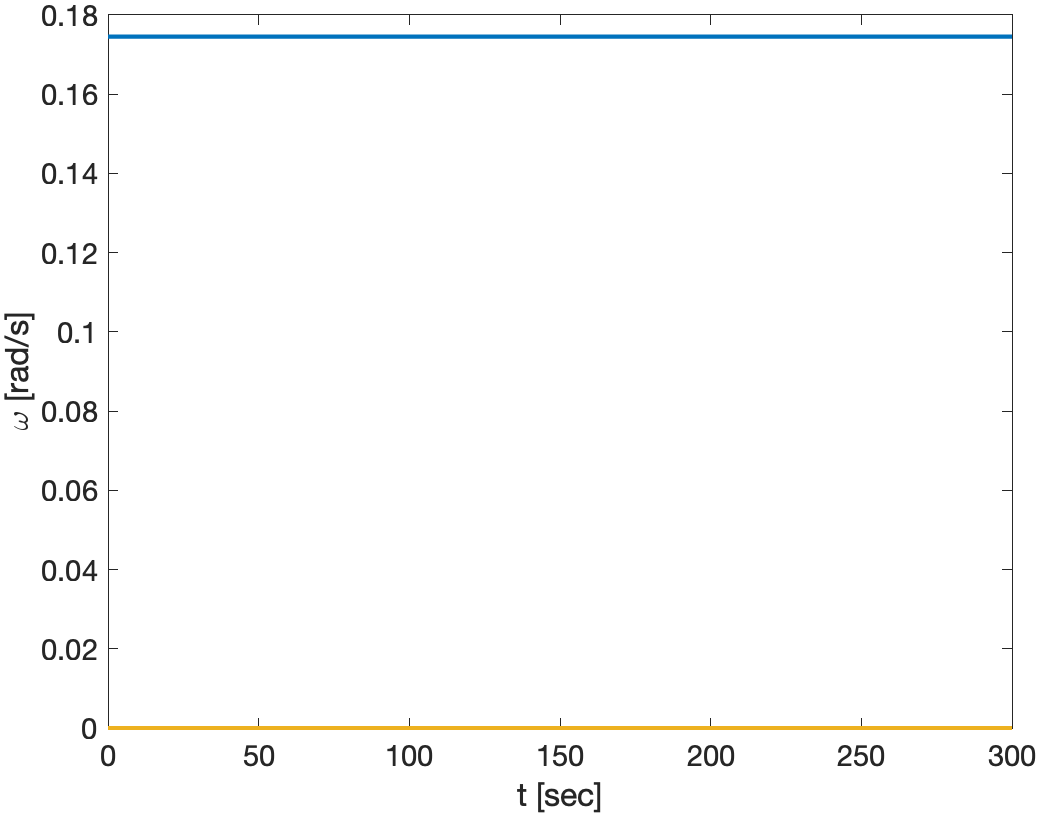
\includegraphics[width = 10cm]{Images/PS4/equilibrium_inertial_velocities.png}
    \caption{Angular Velocity Vector Components Expressed in the Principal Frame for Equilibrium about the X-Axis}
    \label{fig:inertial_equilibrium}
\end{figure}

\subsubsection{Repeat a. by setting the initial attitude to match the RTN frame. Set the initial angular velocity to
be non-zero only about N. Show the evolution of attitude motion in the RTN frame and give an
interpretation of the results (recall that you might have J2 effects in orbit propagation, consider
removing them for verification).}

\subsection{Problem 2 - Stability Tests}

\subsubsection{Pretend you have a single-spin satellite. Set initial conditions to correspond alternatively to the 3
possible equilibrium configurations (rotation about principal axes of inertia). Slightly perturb initial
condition. Is the attitude stable or unstable? In angles and velocities? If stable, periodically or
asymptotically? Show it.}

\subsection{Problem 3 - Adding a Momentum Wheel or Rotor (Dual-Spin Satellite)}

\subsubsection{Re-program Euler equations to include a generic momentum wheel or rotor with rotation axis
aligned with one of the principal axes of inertia. Ideally the wheel or rotor has specs representative
of commercial products (inertia, rotational speed).}

\subsubsection{Numerically integrate Euler AND Kinematic equations from equilibrium initial condition. Verify
that integration is correct as from previous tests (conservation laws, rotations, etc.).}

\subsubsection{Verify equilibrium and its stability similar to previous pset.}

\subsubsection{Use the stability condition to make attitude motion stable for rotation about intermediate moment
of inertia by changing moment of inertia and/or angular velocity of the momentum wheel or rotor.}

\subsubsection{Try to make rotation about another arbitrary axis (potentially relevant to your project) stable
through a generic momentum wheel or rotor.}

\subsection{Problem 4 - Gravity Gradient Torque (Modeling)}

\subsubsection{Remove rotor.}

\subsubsection{Program gravity gradient torque. Feed torque to Euler equations. This is the first perturbation you
model resulting from the interaction of the spacecraft with the environment. Hint: change your orbit
to make gravity gradient significant if that’s not the case.}

\subsubsection{Verify that the magnitude of the modelled torque is consistent with the orbit and inertia tensor of
your satellite. Hint: use simplified formulas from class on modelling of gravity gradient torque.}

\subsubsection{Numerically integrate Euler and Kinematic equations including gravity gradient from initial
conditions corresponding to body axes aligned with the orbital frame (RTN). Verify that gravity
gradient torque is zero, besides numerical errors. Hint: you may need to simplify the orbit to
unperturbed circular to achieve this. Check that initial angular velocity matches mean motion.}

\subsubsection{Numerically integrate Euler and Kinematic equations including gravity gradient from arbitrary
initial conditions (e.g., relevant to your project). Plot external torque (3 components w.r.t. time)
and resulting attitude motion (depends on attitude parameterization, add Euler angles for better
geometrical interpretation) over multiple orbits. Comment on results.}


